\documentclass{article}
\usepackage{tikz}
\usetikzlibrary{arrows.meta,positioning,calc,shapes.geometric}
\pagestyle{empty}
\begin{document}
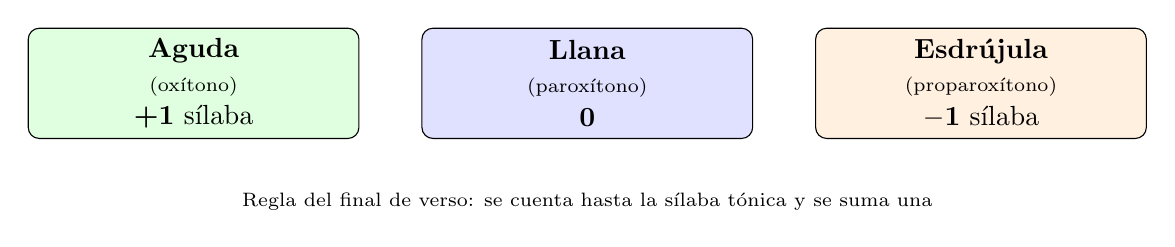
\begin{tikzpicture}
\tikzset{every node/.append style={align=center}}

\node[draw, rounded corners, fill=green!12, minimum width=4.2cm, minimum height=1.4cm, align=center] (a) at (0,0) {\textbf{Aguda}\\ \scriptsize (oxítono)\\ \textbf{+1} sílaba};
\node[draw, rounded corners, fill=blue!12, minimum width=4.2cm, minimum height=1.4cm, align=center] (b) at (5,0) {\textbf{Llana}\\ \scriptsize (paroxítono)\\ \textbf{0}};
\node[draw, rounded corners, fill=orange!12, minimum width=4.2cm, minimum height=1.4cm, align=center] (c) at (10,0) {\textbf{Esdrújula}\\ \scriptsize (proparoxítono)\\ \textbf{$-$1} sílaba};
\node[font=\scriptsize] at (5,-1.5) {Regla del final de verso: se cuenta hasta la sílaba tónica y se suma una};

\end{tikzpicture}
\end{document}
